\chapter{Overlapping, heterogeneous age groups: atrial fibrillation}
\label{applications-age_groups}

Atrial fibrillation research has no standard set of age groups for study.  Therefore the meta-analysis of data from systematic review on the descriptive epidemiology parameters of atrial fibrillation provides an excellent example of overlapping and heterogeneous age groups.

Atrial fibrillation is the most common type of cardiac arrhythmia.  Chaotic and irregular heart rhythms originating in the atria cause poor blood flow to the body.  Atrial fibrillation episodes may be occasional, only lasting a few minutes or hours, or chronic if the heart rhythm is always abnormal.  Symptoms include heart palpitations, lack of energy, dizziness, shortness of breath and chest discomfort, although some cases of atrial fibrillation are symptomless.  Atrial fibrillation may occur at any age with increasing risk for older ages.  It is uncommon in children \cite{rich_epidemiology_2009, rho_asymptomoatic_2005, american_acc_2006, radford_atiral_1977}.

For analysis, atrial fibrillation in Western Europe has 229 rows of data.  As seen from Figure \ref{fig:app-af data}, atrial fibrillation has heterogeneous and overlapping age groups.  Without access to the microdata needed to recreate homogeneous age groups, an alternate approach must be used.  As a solution to the heterogeneous age groups, age-standardizing adds age-weights to the age-specific rate according to population structure.  The age-standardizing model uses a common age pattern for all studies so that the age-weights are the same for all age groups.  Chapter \ref{theory-age_group_model-overlapping_data} offers more details.

    \begin{figure}[h]
        \begin{center}
            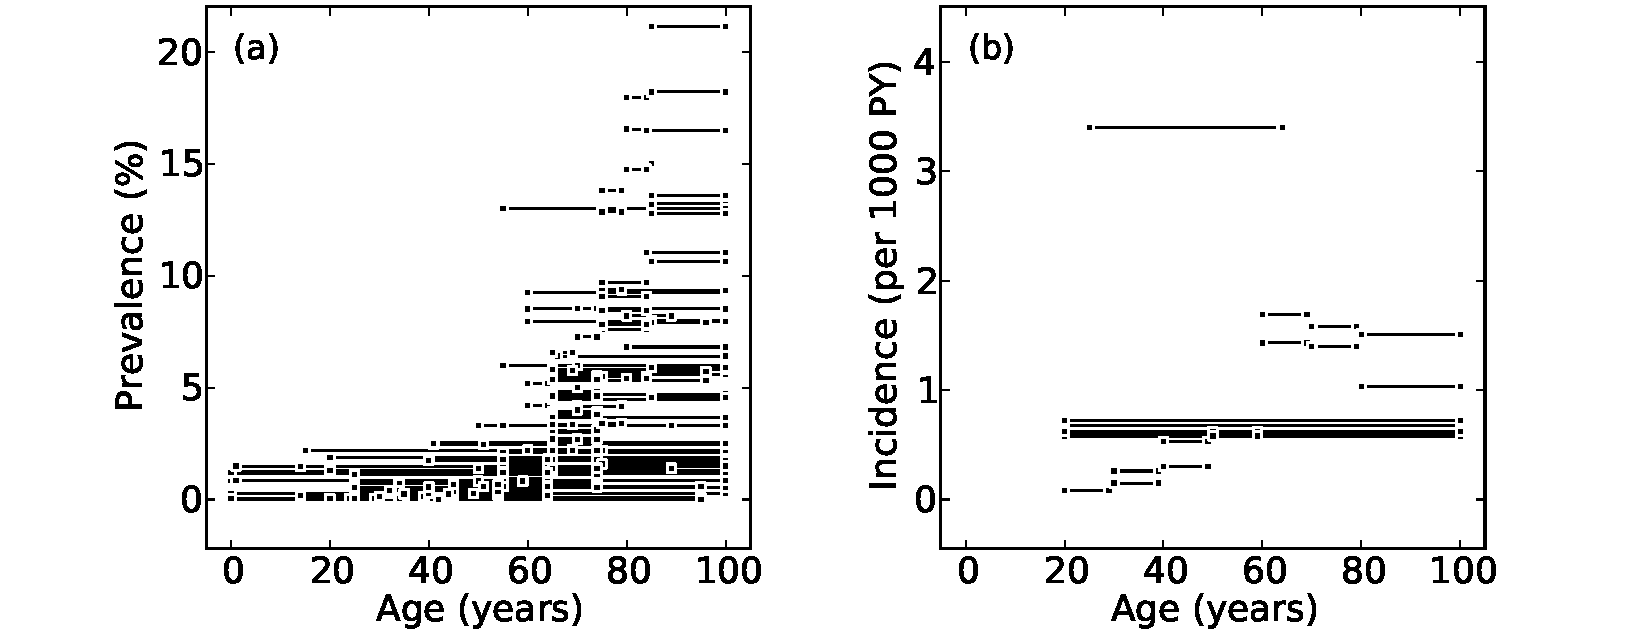
\includegraphics[width=\textwidth]{af-data.pdf}
            \caption{Data for Western Europe males with atrial fibrillation is an excellent example of heterogeneous and overlapping age groups.}
            \label{fig:app-af data}
        \end{center}
    \end{figure}

    \begin{figure}[h]
        \begin{center}
            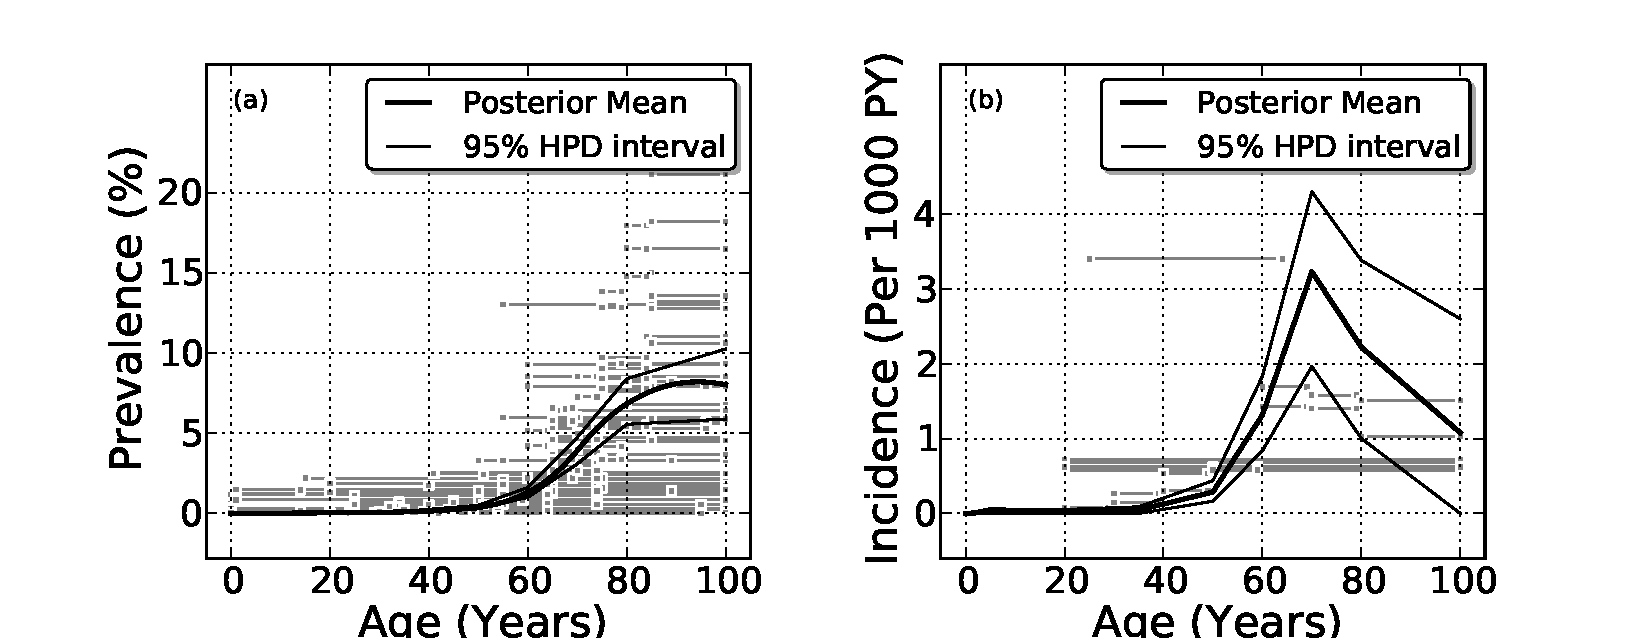
\includegraphics[width=\textwidth]{af-best_model.pdf}
            \caption{Estimates of prevalence and incidence of atrial fibrillation in males in Western European in 1990 using an age-standardizing compartmental model.}
            \label{fig:app-af age-stand}
        \end{center}
    \end{figure}

As discussed in Chapter \ref{theory-age_group_model-overlapping_data}, the simplest approach to modeling heterogeneous age groups is to apply each age-specific rate measurement to the midpoint of the age interval (Figure \ref{fig:app-af mp data}).  However, compared to the age-standardizing method, the midpoint method tends to overestimate as seen in Figure \ref{fig:app-af compare}.

    \begin{figure}[h]
        \begin{center}
            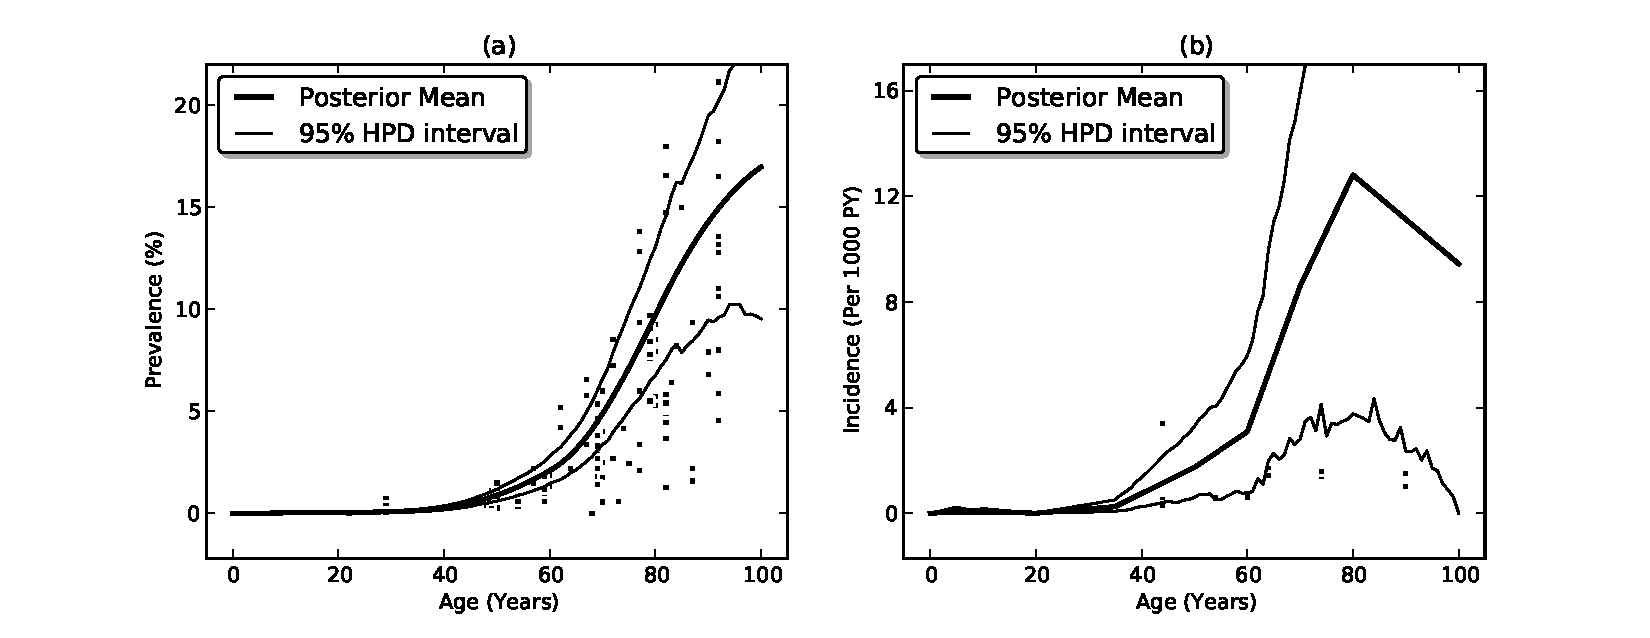
\includegraphics[width=\textwidth]{af-ageless_model.pdf}
            \caption{Using a compartmental model midpoint method, data were fit by applying the age-specific rate to the midpoint of the age group for estimated prevalence and incidence for Western European males with atrial fibrillation in 1990.}
            \label{fig:app-af mp data}
        \end{center}
    \end{figure}

    \begin{figure}[h]
        \begin{center}
            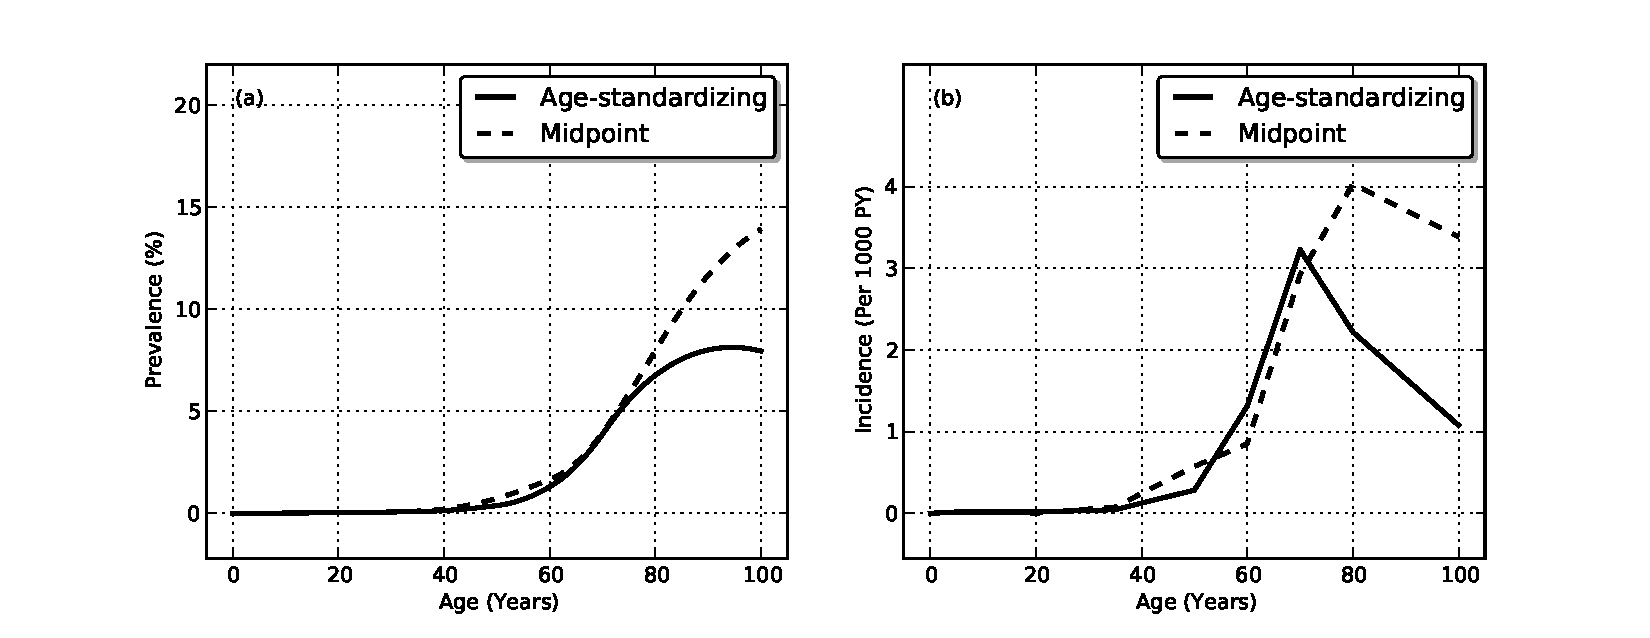
\includegraphics[width=\textwidth]{af-mp_v_hetero.pdf}
            \caption{Comparison of the age-standardizing and midpoint methods for estimated prevalence and incidence for Western Europe males with atrial fibrillation in 1990.}
            \label{fig:app-af compare}
        \end{center}
    \end{figure}
